\documentclass[11pt, oneside]{article} 
\usepackage{geometry}
\geometry{letterpaper} 
\usepackage{graphicx}
	
\usepackage{amssymb}
\usepackage{amsmath}
\usepackage{parskip}
\usepackage{color}
\usepackage{hyperref}

\graphicspath{{/Users/telliott_admin/Dropbox/Tex/png/}}
% \begin{center} 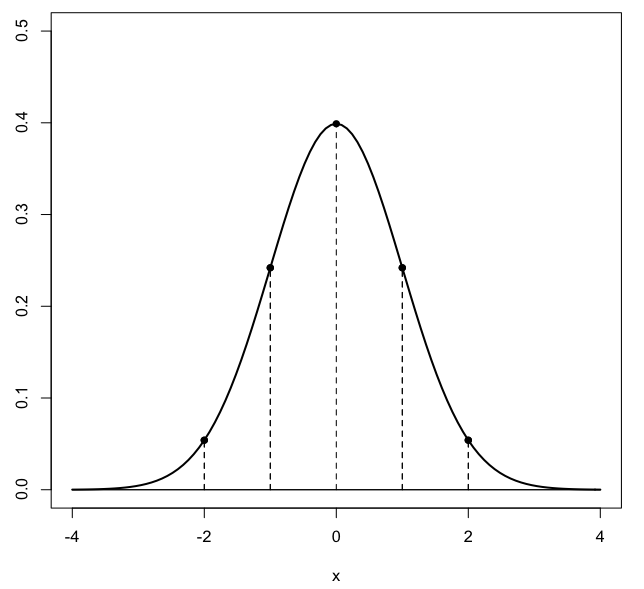
\includegraphics [scale=0.4] {gauss3.png} \end{center}

\title{Pythagorean triples}
\date{}

\begin{document}
\maketitle
\Large

\label{sec:pythagorean_triples}
 
From the chapter on the Pythagorean theorem:
\subsection*{Pythagorean triples}
The triples which are not multiples of another triple are called \emph{primitive}.  For every integer $m,n$, with $m > n$, a Pythagorean triple is given by Euclid's formula:
\[ a = m^2 - n^2 \ \ \ \ b = 2mn \ \ \ \ c = m^2 + n^2 \]

We must choose $m$ and $n$ of opposite parity (one even and one odd).  Otherwise, $a$, $b$ and $c$ will all be even and the triple won't  be primitive.

It is easy to see why this works:
\[ a^2 + b^2 = (m^2 - n^2)^2 + (2mn)^2 \]
\[ = m^4 - 2m^2n^2 + n^4 + 4m^2n^2 \]
\[ = m^4 + 2m^2n^2 + n^4 \]
\[ = (m^2 + n^2)^2 = c^2 \]

\subsection*{all primitive triples}
Maor gives a proof that \emph{all primitive triples} can be found using Euclid's formula.

Consider 
\[ a^2 + b^2 = c^2 \]
For a primitive triple, $a$ and $b$ should be of opposite parity, with one even and one odd.  For if not:

Suppose $a$ and $b$ both even.  Then $a = 2m$ and $b = 2n$ and
\[ a^2 + b^2 = 4(m^2 + n^2) = c^2 \]
Thus $c$ is even and the triple is not primitive.

Otherwise, suppose $a$ and $b$ both odd.  Then $a = 2j +1$ and $b = 2k + 1$ and
\[ a^2 + b^2 = 4j^2 + 4j + 1 + 4k^2 + 4k + 1 = c^2 \]
Hence $c^2$ is even but not divisible by $4$.

On the other hand, if $a$ and $b$ are odd, so are $a^2$ and $b^2$, thus their sum is even.  But if $c^2$ is even, then so is $c$, thus 
\[ (c)^2 = (2i)^2 \]
and $c^2$ must be divisible by $4$.  We have reached a contradiction.  

Therefore only one of $a$ and $b$ is even.  Let $a = 2t$.
\[ (2t)^2 + b^2 = c^2 \]
\[ (2t)^2 = c^2 - b^2 \]
\[ (2t)^2 = (c + b) \cdot (c - b) \]
\[ t^2 = \frac{c+b}{2} \cdot \frac{c - b}{2} \]

Since $a^2$ is even and $b^2$ is odd, $c^2$ is odd, so $c$ is also odd.  

Therefore the sum $c+b$ and difference $c-b$ are both even.  This means that the terms on the right-hand side in the last expression above are integers.

$b$ and $c$ are also both relatively prime.  If they were not, then the sum and difference would share this factor and the same factor would also be shared by $a$, contrary to the assumption that this is a primitive triple.

The left-hand side 
\[ t^2 = \frac{c+b}{2} \cdot \frac{c - b}{2} \]
is a perfect square, so the right-hand side is also.  

On the right, since the two terms are relatively prime, each term must itself be a perfect square, otherwise their product would not be a perfect square.

So we can write:
\[ u^2 = \frac{c + b}{2}  \]
\[ v^2 = \frac{c - b}{2}  \]

Adding the two equations we obtain
\[ u^2 + v^2 = c^2 \]
Since $c$ and $c^2$ are both odd, this shows that $u$ and $v$ have \emph{opposite} parity.  Subtracting
\[ u^2 - v^2 = b^2 \]
Finally
\[ t^2 = u^2 v^2  \]
\[ t = uv \]
\[ a = 2t = 2uv \]

There is a small table of triples in this discussion of Euclid X:29 by Joyce:

\url{https://mathcs.clarku.edu/~djoyce/elements/bookX/propX29.html}

\begin{center} 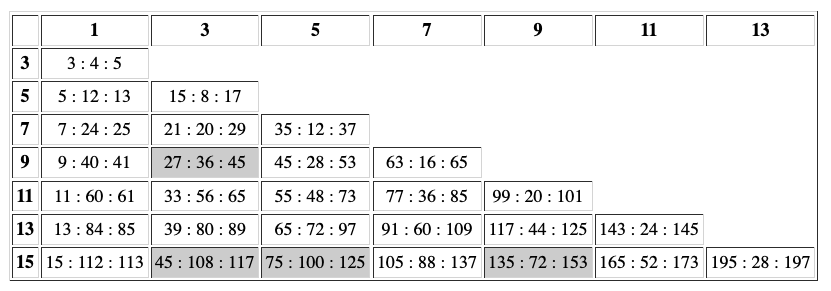
\includegraphics [scale=0.5] {triples_joyce.png} \end{center}

\subsection*{code}

Here is a Python script to generate triples by exhaustive search:

\url{https://gist.github.com/telliott99/b543f41d84155bc9171df68b6350e256}

And here is one that implements Euclid's formula:

\url{https://gist.github.com/telliott99/144c1a7e90740eb1614ca8ceb5bdeed9}

Here is some output ($m,n,a,b,c$) from the second script, sorted on $m$ and $n$:

\begin{verbatim}
> python triples2.py
  1   2   3   4   5 
  1   4   8  15  17 
  1   6  12  35  37 
  1   8  16  63  65 
  1  10  20  99 101 
  1  12  24 143 145 
  1  14  28 195 197 
  2   3   5  12  13 
  2   5  20  21  29 
  2   7  28  45  53 
  2   9  36  77  85 
  2  11  44 117 125 
  2  13  52 165 173 
  3   4   7  24  25 
  3   8  48  55  73 
  3  10  60  91 109 
  3  14  84 187 205 
  4   5   9  40  41 
  4   7  33  56  65 
  4   9  65  72  97 
  4  11  88 105 137 
  4  13 104 153 185  not in list
...
\end{verbatim}

To test triples for being primitive, we look for a greatest common divisor of $a$ and $b$ equal to $1$.  All such triples have $m$ and $n$ of opposite parity.

The last entry says "not in list" because the limit set for the exhaustive search was exceeded.  With a larger search, this triple would be found (or it can just be confirmed by direct computation).

When sorted on $a,b,c$ all triples found by exhaustive search appear to also be found by Euclid's formula, but this wasn't tested explicitly.  That could be done easily, as an exercise.

There are some interesting patterns in lists of triples.  Here are two:

\begin{verbatim}
   3    4    5 
   5   12   13 
   7   24   25 
   9   40   41 
  11   60   61 
  13   84   85 
  15  112  113 
  17  144  145 
  19  180  181 
  21  220  221 
  23  264  265 
  25  312  313 
  27  364  365 
\end{verbatim}

The first entry doesn't fit the pattern.  But starting with $5,12,13$, for every step $\Delta a = 2$, we get $\Delta b$ increasing in steps of $4$, with $c = b + 1$.

Below, starting with $8,15,17$, for every step $\Delta a = 4$, we get $\Delta b$ increasing in steps of $8$, with $c = b + 2$.

\begin{verbatim}
   8   15   17 
  12   35   37 
  16   63   65 
  20   99  101 
  24  143  145 
  28  195  197 
 \end{verbatim}

\end{document}